\documentclass[sigconf,anonymous,natbib=false,10pt]{acmart}
\hyphenation{pseu-do-ny-mi-za-tion pseu-do-ny-mizes sche-mas}
\settopmatter{printacmref=false}
\setcopyright{none}
\renewcommand\footnotetextcopyrightpermission[1]{}

\acmConference[HotOS '25]{Workshop on Hot Topics in Operating Systems}{May
2025}{Banff, Alberta, Canada}


%\begin{CCSXML}
%<ccs2012>
%   <concept>
%       <concept_id>10002978.10003029.10011703</concept_id>
%       <concept_desc>Security and privacy~Usability in security and privacy</concept_desc>
%       <concept_significance>300</concept_significance>
%       </concept>
%   <concept>
%       <concept_id>10002951.10002952.10003190</concept_id>
%       <concept_desc>Information systems~Database management system engines</concept_desc>
%%       <concept_significance>300</concept_significance>
%       </concept>
% </ccs2012>
%\end{CCSXML}

%\ccsdesc[300]{Security and privacy~Usability in security and privacy}
%\ccsdesc[300]{Information systems~Database management system engines}

% to be able to draw some self-contained figs
\usepackage{tikz}
\usepackage{amsmath}
\usepackage{hyperref}
\usepackage[normalem]{ulem}
\usepackage{listings}
\usepackage{xspace}
\usepackage{booktabs}
\usepackage{multirow}
\usepackage{wasysym}
\usepackage{caption}
\usepackage{subcaption}
\usepackage{enumitem}
\usepackage[utf8]{inputenc}
\usepackage[compact, small]{titlesec}
\usepackage{algorithm}
\usepackage{algpseudocode}

\captionsetup{labelfont=bf,textfont=rm,belowskip=-8pt,aboveskip=4pt}

% BibLaTeX for bibliography
\usepackage[
  backend=biber,
  style=numeric-comp,
  minalphanames=3,
  isbn=false,
  sortcites=true,
  sorting=anyt,
  abbreviate=false,
  url=false,
  doi=false,
  maxnames=99,
  minbibnames=3,
  maxbibnames=99]{biblatex}
\addbibresource{paper.bib}

\AtBeginBibliography{\small}
\setcounter{biburllcpenalty}{7000}
\setcounter{biburlucpenalty}{8000}

\newcommand\ms[1]{\textcolor{red!55!blue}{[malte: {#1}]}}
\newcommand\hmng[1]{\textcolor{blue!40!red}{[hmng: {#1}]}}
\newcommand\lyt[1]{\textcolor{green!55!blue}{[lyt: {#1}]}}
\newcommand\eddie[1]{\textcolor{blue!55!blue}{[E: {#1}]}}
\newcommand{\tabitem}{~~\llap{\textbullet}~~}
\newcommand{\eg}{{e.g.},\xspace}
\newcommand{\ie}{{i.e.},\xspace}

\newcommand{\one}{({\em i}\/)}
\newcommand{\two}{({\em ii}\/)}
\newcommand{\three}{({\em iii}\/)}
\newcommand{\four}{({\em iv}\/)}
\newcommand{\five}{({\em v}\/)}
\newcommand{\six}{({\em vi}\/)}

\newcommand{\sys}{XX}

\definecolor{codegreen}{rgb}{0,0.4,0}
\definecolor{codegray}{rgb}{0.5,0.5,0.5}
\definecolor{codepurple}{rgb}{0.58,0,0.82}
\definecolor{backcolour}{rgb}{0.95,0.95,0.92}

\lstdefinestyle{rust}{
    %backgroundcolor=\color{backcolour},
    commentstyle=\color{codegreen},
    keywordstyle=\color{codepurple},
    stringstyle=\color{blue},
    basicstyle=\ttfamily\scriptsize,
    breakatwhitespace=false,
    breaklines=true,
    captionpos=b,
    keepspaces=true,
    showspaces=false,
    showstringspaces=false,
    showtabs=false,
    tabsize=2
}
\lstset{style=rust}

%-------------------------------------------------------------------------------
\begin{document}
%-------------------------------------------------------------------------------

%don't want date printed
\date{}

%%
%% The "title" command has an optional parameter,
%% allowing the author to define a "short title" to be used in page headers.
% make title bold and 14 pt font (Latex default is non-bold, 16 pt)
\title{\sys{}: A system}

%%
%% The "author" command and its associated commands are used to define
%% the authors and their affiliations.
%% Of note is the shared affiliation of the first two authors, and the
%% "authornote" and "authornotemark" commands
%% used to denote shared contribution to the research.

\author{
{\rm Anonymous Authors}\\
} % end author

%\author{Hannah Gross}
%\affiliation{%
  %\institution{Brown University}
%\email{tslilyai@mit.edu}
%\affiliation{%
%  \institution{MIT}
%  \state{}
  %\country{}
%}

%\author{Lillian Tsai}
%\affiliation{%
  %\institution{MIT CSAIL}
%\email{tslilyai@mit.edu}
%\affiliation{%
%  \institution{MIT}
%  \state{}
  %\country{}
%}

%\author{Eddie Kohler}
%\affiliation{%
  %\institution{Harvard University}
%\email{kohler@seas.harvard.edu}
%\affiliation{%
%  \institution{Harvard University}
%  \state{MA}
  %\country{}
%}

%\author{Malte Schwarzkopf}
%\affiliation{%
  %\institution{Brown University}
%\email{malte@cs.brown.edu}
%\affiliation{%
%  \institution{Brown University}
%  \state{RI}
  %\country{}
%}

\begin{abstract}
    
    Serverless is in principle a good match for web applications, allowing
    developers to pay for the resources needed as load varies without having to
    reserve servers.

    This paper identifies the crowding problem, where under high total load,
    different tenants’ functions compete for resources, and thus can drive up each
    other’s delays. Because of this problem, existing serverless designs result in
    latencies that are not tolerable for user-facing functions, even in systems that
    have fast function start time.

    We argue for new a design based on price classes that can keep the latency of
    high price class functions stable even under high load, making it feasible to
    run web applications as functions.

\end{abstract}


\maketitle

%-------------------------------------------------------------------------------
\section{Introduction}
%-------------------------------------------------------------------------------

A world where all cloud compute is run in the format of serverless jobs is
attractive to developers and providers: developers pay only for what they use
while having access to many resources when needed; and cloud providers have
control over scheduling and can use that to drive up utilization.


However, for many applications it is rare to see them entirely hosted on
serverless offerings today\cite{TODO}. Consider a web server: its
characteristics of unpredictable and bursty traffic make it well-suited for
serverless, and the pay as you go model is particularly attractive to website
developers who don't want to have to worry about provisioning.

Suppose a simple web server consists of two different page views, one for the
landing page and another for users' profile pages, and also has map reduce jobs
for data processing. It is important that the page views finish quickly, with
the landing page taking precedence over the profile pages, and the map reduce
jobs can be run in the background and be delayed.

If a web developer wanted to host their web in an existing serverless offering,
a popular option is AWS lambda\cite{TODO}. However, AWS offers no way to
distibguish between different lambdas in terms of their priority. A developer
using AWS lambda could use cold start avoidance mechanisms (such as reserved
concurrency) for higher priority functions; or giving them more concurrency
(through `vCPUs'), but neither of these give real priority to the
functions.\hmng{that is not on the nose}

This paper focuses on building a usable and efficient scheduling mechanism to
support differentiating between jobs of different priorities in a world of
universal serverless. In doing so, it faces multiple significant challenges.

One of the challenges is that of placing jobs quickly enough. This means that a
job that takes 20ms to run cannot spend 100ms in scheduler queues and waiting
for an execution environment before even starting to run. One part of this
challenge is cold starts. For this paper, we assume that that generally cold
start times are small enough compared to the jobs being run that cold starts on
the critical path are acceptable.\footnote{Cold start latencies are a popular
area of research and as a result have been reduced significantly --- recent
state of the art systems have been able to support latencies in the single digit
ms range\cite{TODO}.} We focus on the aspect of scheduling latency: in a
datacenter, where both the number of new jobs coming in and the amount of
resources are extremely large, the challenge is knowing where the free and idle
resources are, or finding out quickly.

Another challenge is that of multi-tenancy. The fact that page views are more
important to a web server than map reduce jobs is a relative statement: there is
no way of mapping that prioritization to other peoples jobs, in order to be able
to directly compare which job should run when. And, in fact, developers cannot
be trusted to make such a comparison, their own jobs will always seem more
important than others': if given an absolute scale from 0-99 (0 being the
highest priority), the highest priority job will always get a 0 and the rest
will be relative to that. However, that does not reflect that in fact different
clients do have different requirements and expectations, and need to be treated
differently.

A third main challenge is that of managing memory. Given that machines are
limited in memory, placing a new high priority job invocation on a machine
already running many jobs may or may not lead to enough memory pressure to
require killing an already placed job (rather than just preempting other jobs).
It is difficult to know whether that would be the case, and if so whether it is
worth it, or better to just requeue the new job.\hmng{I think this challenge is
a little weak; I should work it out more}

 

\section{Approach \& Design}\label{design}

Our approach addresses the variability of runtimes, which is undesirable for
latency sensitive functions, by using \priceclass{}es as a metric to tell \sys{} what
to prioritize and what not. We will show that this allows us to stabilize the
runtimes for the high \class{} functions. 

In fact, \sys{} uses \class{}es to supplant the current interface, which
requires developers choose an amount of memory per function, which is then tied
to a cpu power (a potentially fractional amount of vCPUs). \Priceclass{}es are
the only thing that developers need to give \sys{}, they pay for memory
separately, and only for what they use. The price for memory is the same across
all \class{}es. This serves the purpose of extending the serverless on-demand
structure to include memory, and moves away from the usual bin packing with
overprovisioning problem.

\Priceclass{}es are a metric that has a number of benefits over resource
reservations. One is that developers are more likely to have a good sense of
what \priceclass{} a function should have ahead of time, because they know in
what context the function will be used and how important it is that the function
run quickly. \Priceclass{}es also remain the same across different invocations,
whereas the resources needed can be heavily skewed in a web server environment,
where popularity distributions are often very
uneven~\cite{hermod,serverless-in-the-wild}. And finally, \class{}es more
directly align the interests of the developer with those of the provider by
communicating on the level of what the provider and developer actually care
about: money, and latency (as achieved by \class{}es in the system).

However, having \priceclass{}es also means that there are no absolute guarantees
about what developers are receiving when they put a price on a function they
want to run. In order to mitigate that somewhat and avoid the developer-side
uncertainty of bidding wars, \sys{} exposes a fixed set of \priceclass{}es. This
is similar to how AWS has different EC2 instance types, that are directly mapped
to prices. Rather than being a guarantee, the \priceclass{} is instead a metric
to express priority to \sys{}, which it can then use to enforce a favoring of
high class functions.

This also allows the provider to provision their datacenters on the level of the
amount of hardware they buy: by looking at the historical overall amount of high
\priceclass{} workload, they know how much hardware they at least need to buy in
order to be able to comfortably fit all of that load.


At the same time, \class{}es give \sys{} the information it needs to decide what
to schedule when. How exactly it does this is what we explore in \sys{}'s design
and evaluation.



\subsection{Interface}


Developers using \sys{} write function handlers and define triggers just like
they would for any existing serverless offering. In addition, each place where
they trigger the function, they assign that invocation to a \priceclass{}. For
instance, a simple web server might consist of a home page view that is assigned
a higher \priceclass{} and costs 2$\mu\cent$ per cpu second, a user profile page
view which is assigned a middle-high \class{} and cost 1.5$\mu\cent$ per cpu
second, and finally an image processing function that can be set to a low
\class{} which costs only 0.5$\mu\cent$ per cpu second.

\Class{}es are inherited across call chains: if a high \class{} function calls a
low \class{} function, that invocation with run with high \class{}. This is
important in order to avoid priority inversion.

To avoid unexpected costs in the case of for example a DOS attack or a bug,
developers also express a monthly budget that they are willing to pay.\ \sys{}
uses this budget as a guideline and throttles invocations or decreases quality
of service in the case that usage is not within reason given the expected
budget, though it does not guarantee that the budget will not be exceeded by
small amounts.



\subsection{\Sys{} Design}

\begin{figure}[t]
    \centering
      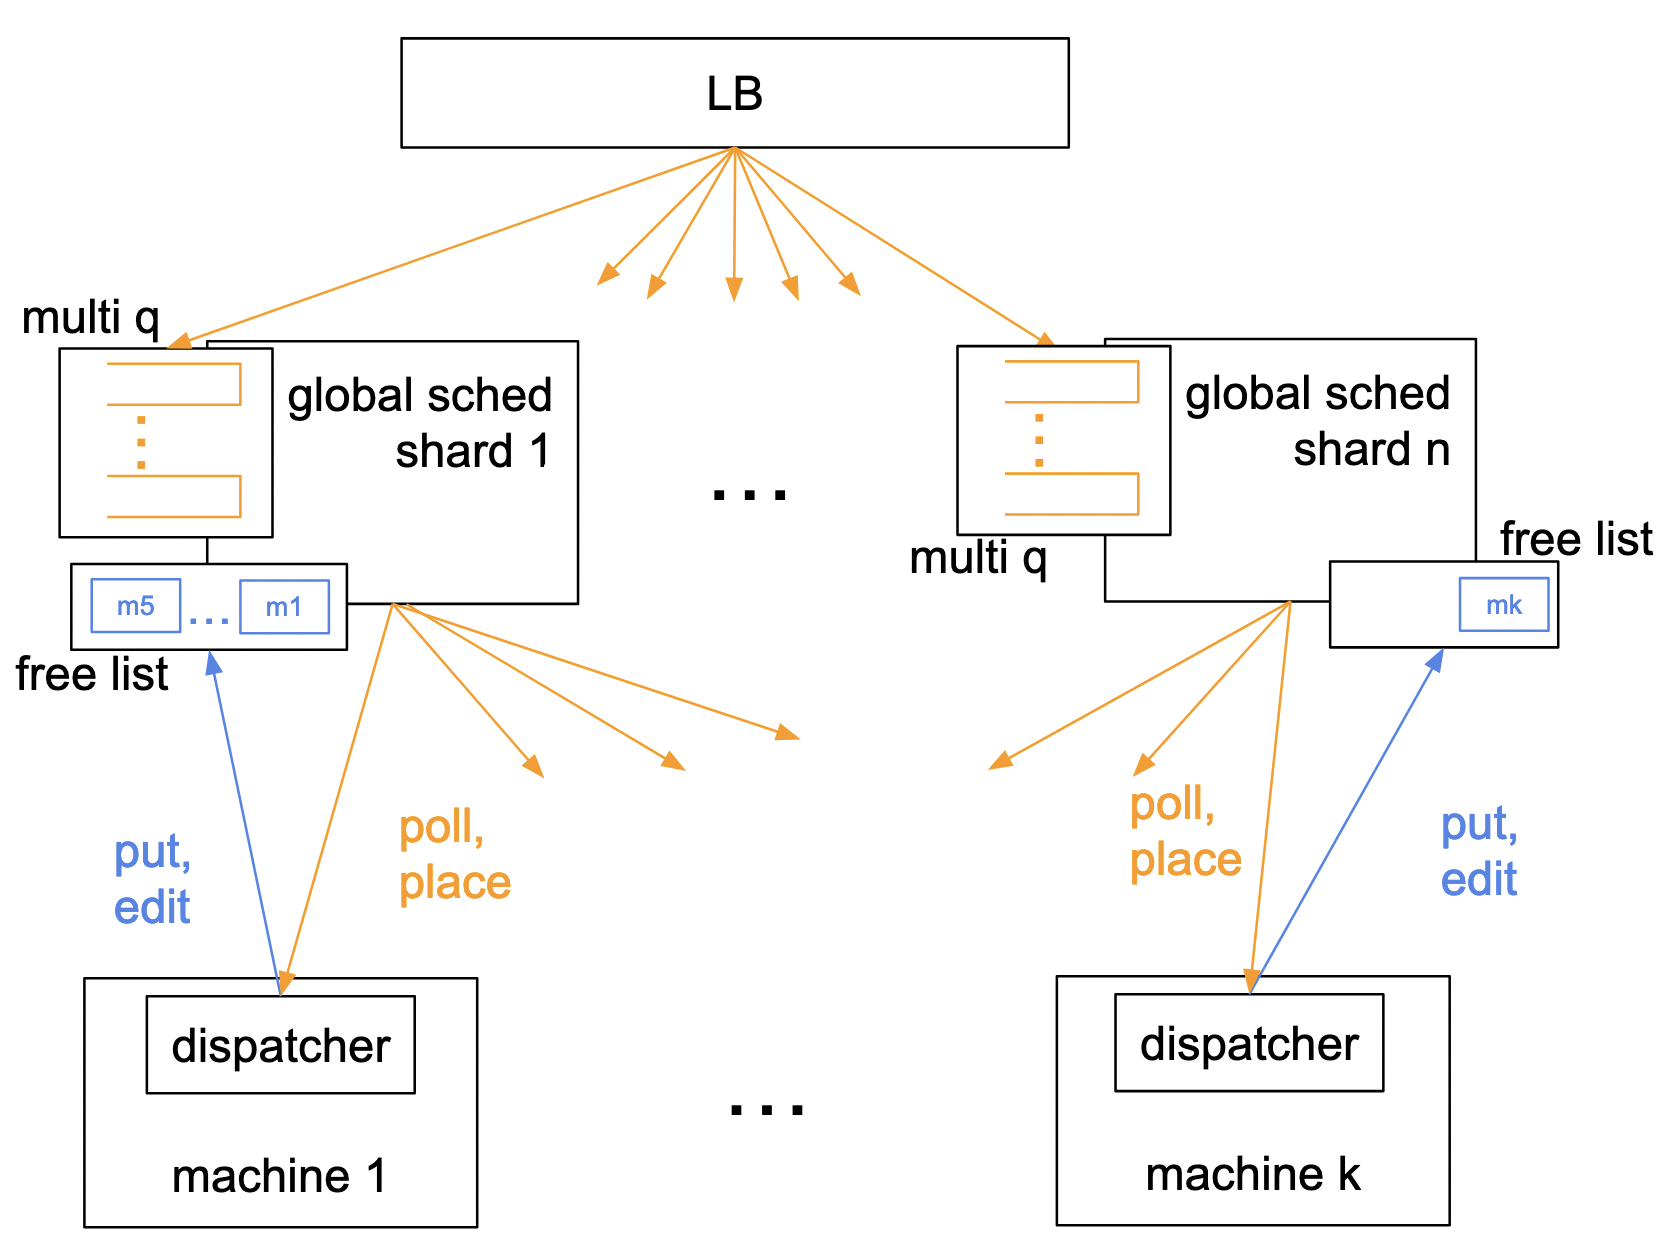
\includegraphics[width=9cm]{img/overview.png}
      \caption{ global scheduler shards queue and place functions (in orange), 
      on each machine a dispatcher thread keeps track of memory utilization 
      and if it's low writes itself to an idle list (in blue) }
    \label{fig:overview}
\end{figure}



\Sys{} has as its goal to enforce the \class{}es attached to functions, which
means it needs to prefer higher \class{} functions over lower ones, and preempt
the latter when necessary.
  

As shown in Figure~\ref{fig:overview}, \sys{} sits behind a load balancer, and
consists of: a \textit{distributed global scheduler}, which places new function
invocations and has attached an \textit{idle list}, a \textit{dispatcher},
which runs on each machine and communicates with the global scheduler shards,
and a \textit{machine scheduler}, which enforces \class{}es on the machines.


\textbf{Machine Scheduler.}
The machine scheduler is a preemptive priority scheduler: it preempts lower
\class{} functions to run higher \class{} ones. Being unfair and starving low
\class{} functions is desirable in \sys{}, since image processing functions
should not interrupt a page view request processing, but vice versa is expected.
Within \class{}es the machine scheduler is first come first served. This matches
Linux' `SCHED FIFO' scheduling~\cite{linux-sched}.


\textbf{Idle list.}
Each global scheduler shard has an idle list, which holds machines that have a
significant amount of memory available. In the shards idle list each machine's
entry is associated with the amount of free memory as well as the current amount
of functions on the machine. The idle list exists because datacenters are large:
polling a small number of machines has been shown to be very powerful, but
cannot find something that is a very rare occurrence~\cite{join-idle-queue}.
Having an idle list allows the machines that have actually idle resources, which
are expected to be rare in a high-utilization setting, to make themselves
visible to the global scheduler. The idle list also allows the global scheduler
to place high \class{} functions quickly, without incurring the latency
overheads of doing the polling to find available resources. This design is
inspired by join idle queue~\cite{join-idle-queue}, but defines idleness via
memory availability rather than empty queues.


\textbf{Dispatcher.}
The dispatcher is in charge of adding itself to a shard's idle list when memory
utilization is low. The dispatcher chooses which list to add itself to using
power-of-k-choices: it looks at k shards' idle lists and chooses the one with
the least other machines in it. If the machine is already on an idle list on
shard $i$, but the amount of available memory has changed significantly (either
by functions finishing and memory being freed or by memory utilization
increasing because of new functions or memory antagonists), the dispatcher will
update shard $i$'s idle list. These interactions from the dispatcher to free
lists are represented by the blue arrows in Figure~\ref{fig:overview}.

The dispatcher is also in charge of managing the machine's memory. When memory
pressure occurs, the dispatcher uses \textit{\class{}-based swapping} to move
low \class{} functions off the machine's memory. In this scenario, having
priority scheduling creates the opportunity that enables this to be realistic:
because the dispatcher knows that the lowest \class{} functions will not be run
until the high \class{} functions have all finished, it can swap its memory out
knowing it will not be needed soon. The dispatcher swaps the low \class{}
function back in when the memory pressure is gone and the function will be
run.\footnote{Whether Linux will simply do the right thing, or require heavy
hinting and guidance from the dispatcher, is an open question in \sys{}'s
design.}

Bounding the amount of swap space required without bounding the amount of memory
that functions can use is not possible. The goal of the dispatcher is to swap
when possible, and in the case that that is not enough it can resort to killing.
Providers can estimate the amount of swap space required by looking at memory
utilization, and since swap space is cheap~\cite{ssd-price} can provision it so
that killing is very rare.

\textbf{Global Scheduler Shards.}
Global scheduler shards store the functions waiting to be placed in a multi
queue, with one queue per \priceclass{}. Shards choose what function to place
next by looking at each function at the head of each queue, and comparing the
ratio of \class{} to amount of time spent in the queue. This ensures that high
\class{} functions don't have to wait as long as low \class{} functions to be
chosen next, but low \class{} functions will get placed if they have waited for
a while.

When placing the chosen function, the shard will first look in its idle list. If
the list is not empty, it will choose the machine with the smallest queue
length.

If there are no machines in the idle list, the shard switches over to
power-of-k-choices: it polls k machines, getting the amount of functions running
from each. The shard then places the new function on the machine with the
smallest number of currently running functions. 

%-------------------------------------------------------------------------------
\section{Preliminary Results}
%-------------------------------------------------------------------------------

% To understand the dynamics of the single machine scheduler, we implement a
% prototype that uses linux' SCHED-FIFO to enforce priorities.\hmng{ also talk about
% options that we thought about in terms of EEVDF/EDF, nice values, etc? Might
% come out of nowhere given that this wasn't a huge deal in the design, but on the
% other hand it is what I've spent the most time on }

% < graph 1: representative microbench comparing straight CFS linux vs cgroups vs nice values vs priority >

To model the whole systems' dynamics, we built a simulator.\hmng{List assumptions and variables?}

< graph 2: graph of latency (and matching graph of utilization?) as load increases; per priority >


%-------------------------------------------------------------------------------
\section{Discussion}
%-------------------------------------------------------------------------------

In this section we discuss the the way that having priorities would impact how
we can approach some of the open questions that remain about how a scheduler
should best manage resources.


\subsection{Managing memory}

In section~\ref{design}, \sys{} makes decisions based on maximum memory usage
estimates for each job, provided by the developer. However, in reality, making
scheduling decisions based off of this sort of estimate of a maximum can lead to
under-utilization. Jobs often have highly variable memory usage; for instance the
distribution of content among users of social media platforms is notoriously
skewed\cite{TODO}, so jobs that fetch information for a user and process it will
be run over very different amounts of data depending on who the user is. So
making scheduling decisions based off of an estimate of a maximum will lead to
memory under-utilization, and instead we are forced to play a game of
overprovisioning.

Having priorities can help. We overprovision in order to achieve high
utilization, so need a way of dealing with a situation where there are not
enough resources for all the jobs on a machine. Under that situation of high
memory pressure, we suggest a priority-based paging approach, where the lower
priority jobs' memory are paged out. Because machines run highest priority first
scheduling, we know that the paged job will not be run until the higher priority
jobs have finished (and thus freed their memory).\hmng{there's a caveat here
where they could block on i/o, but the likelihood that all the jobs except the
last one block on i/o is low} Later, when there is lower load, and the
previously paged job is ready to run again, the machine can page back in all of
its memory. Thus the paged job pays no latency overhead for having been paged,
and the amount of time spent paging memory is low: once to move all the memory
out, and once to move it back in. This is the minimal amount of data movement
necessary to free up the required memory without deleting/killing.


% One option is profiling: as ML models improve, so our ability to predict things
% improves, including predicting memory usage. Especially for jobs with a high
% variance of memory usage, using a model that is given the inputs to invocations
% could work well, since the inputs are likely to be the determining factor for
% memory usage (for instance, the model could learn which users are the ones that
% have huge amounts of data). However, predictions are still just estimates that
% could always be wrong, and the system needs to be able to handle that. They also
% need to be based on profiling information, which will be slow to adapt to
% changes in code and in the underlying data.

% Another option is snapshotting: lower priority functions are allowed to snapshot
% themselves and then are placed somewhere else and re-started. This way none of
% their already done computation is wasted, and the memory is freed. However, the
% timescale would have to be such that the snapshotting does not (in its use of
% memory or compute) prohibitively block the other jobs on the machine from
% running. This works against the incentives of the situation: ideally we want to
% free a large amount of memory, but the time it takes to snapshot a job scales
% with the amount of memory it is using.


\subsection{Managing compute}

We have already seen that having priorities helps \sys{} deal with
overprovisioning on the compute side. Traditionally, managing the response time
for important jobs requires the overall load on the system to be low, because
slowdown is averaged across all the jobs that can share resources. However,
having priorities allows \sys{} to be targeted about how compute resources are
shared: rather than averaging out the slowdown caused by overprovisioning across
all the jobs by having them time share the cores, \sys{} can use priorities to
decide which job has to wait. This means that in priority scheduling the amount
of time a job spends waiting for resources is only defined by the load of jobs
with equal or higher priority.

The flipside of this is that it is possible that the entire load of the
datacenter will be such that low priority jobs are starved. This is acceptable
and in fact desirable for small amounts of time, but keeping this effect in
check requires managing the overall load. 

We propose to solve this problem by ensuring that it can never be the case the
there is so much load on high priority jobs that the data center will be full
with them to such a degree that other jobs can't run. There is evidence for and
we expect that load on a high level will mostly be stable, with diurnal and
annual patterns.\cite{TODO}

This means that providers can mostly choose the rough breakdown of the load they
will have at any given time (ie they can choose a percentage of how many jobs
they want in each priority, and change it by adjusting prices or not allowing
users to select that level anymore). 



\section{Related Work}

Many other projects have explored how to do better scheduling for data centers.
 
Systems like Sparrow\cite{sparrow}, Hermod\cite{hermod}, or Kairos\cite{kairos}
improve performance of scheduling in the distributed setting by trying out and
using different scheduling policies. Unlike \sys{}, they treat all functions
equally.

Some approaches are directly tailored for serverless.

Some systems generate information about functions themselves to help placement
decisions; for instance ALPS\cite{alps}, which observes and learns the behaviors
of existing functions and then makes scheduling decisions based on those; or
Morpheus\cite{morpheus}, which learns SLOs from historical runs, and then
translates these to recurring reservations.~\Sys{} instead gets the \class{}es
directly from the developers as part of its interface.


Other papers have taken the same approach as \sys{} of getting information to
help scheduling from the developers. Sequoia\cite{sequoia}, for instance,
creates a metric of QOS for serverless functions. Unlike \sys{} however, Sequoia
does not implement a new scheduler, but is itself a serverless function that
manages the invocation sequence of developer's function chains by interposing on
the triggers and choosing what to invoke when. Therefore it also, unlike
\sys{}, does not support multi-tenancy.

Another project\cite{app-paper} creates a language of Allocation Priority
Policies (APP), which is a declarative language to express policies, then builds
a scheduler around that. The APP language is built around allowing developers to
specify custom load balancing decisions, and the scheduler uses the developers'
specification to define a mapping of function invocations to workers. 


%-------------------------------------------------------------------------------
%\bibliography{paper.bib}
\printbibliography

%%%%%%%%%%%%%%%%%%%%%%%%%%%%%%%%%%%%%%%%%%%%%%%%%%%%%%%%%%%%%%%%%%%%%%%%%%%%%%%%
\end{document}
%%%%%%%%%%%%%%%%%%%%%%%%%%%%%%%%%%%%%%%%%%%%%%%%%%%%%%%%%%%%%%%%%%%%%%%%%%%%%%%%

%%  LocalWords:  endnotes includegraphics fread ptr nobj noindent
%%  LocalWords:  pdflatex acks
